%% chapter 2

\chapter{相关工作}

\section{单细胞测序}
  生物体内各种组织之间存在巨大的差异,甚至同一块组织也会有在形态、功能上差异巨大的细胞。Bulk-RNA测序技术可以很好地用来探究组织之间的异质性,但其无法很好地解决后面一个问题,其原因便在于Bulk-RNA测序技术无法提供单细胞层级的转录信息。相较之下,单细胞RNA测序(scRNA-seq)技术提供了在单细胞水平观测基因表达的方法,可以更好地研究组织内的细胞异质性\cite{hammond2019single,keren2017unique,li2019developmental,masuda2019spatial,masuda2020novel,matcovitch2016microglia}。

\begin{figure}[!htb]
  \centering
  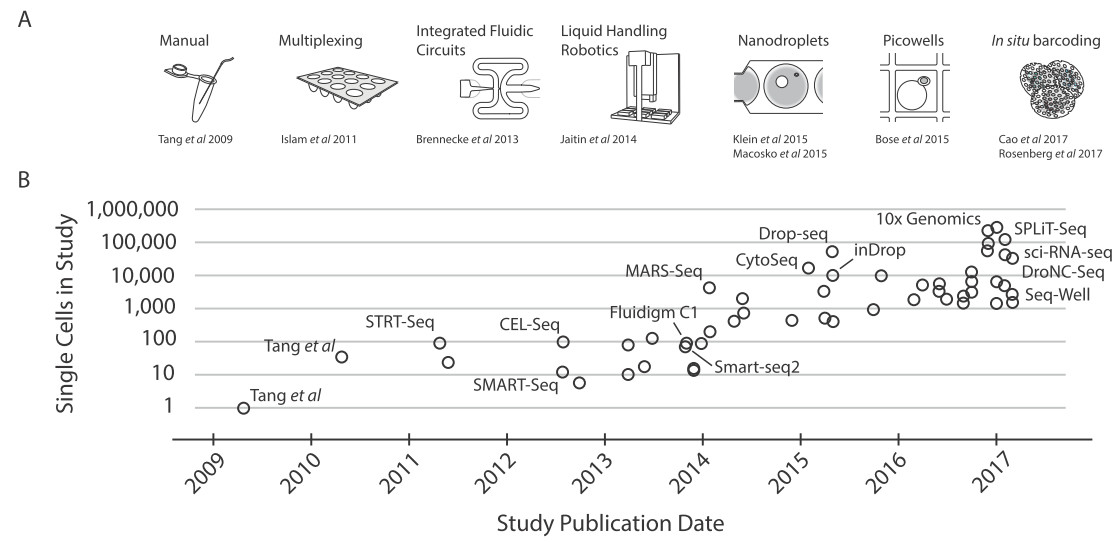
\includegraphics[width=0.8\textwidth]{figs/scseq-development.jpeg}
  \caption{单细胞测序技术近年来的发展}
  \label{fig:scseq-development}
\end{figure}

  单细胞测序技术最初起始于Kurimoto等人在2006年的一项工作\cite{kurimoto2006improved},这项工作对于后来单细胞转录组测序的原理发展有很大的影响。该研究主要特点在于加入了T7启动子,这样便把cDNA为期29个循环的扩增切分为两段,减少PCR扩增的偏差。汤富酬等人在2009年所做的一项工作\cite{tang2009mrna},延用了Kurimoto等人在2006年工作\cite{kurimoto2006improved}中在末端加A的思路。但是在最后读取cDNA信息的时候,汤等人使用了Applied Biosystem的二代测序SOLiD system平台,也就是取代了芯片的读取方式。

  目前应用最广泛的是模板转换法,主要代表技术便是SMART-seq\cite{ramskold2012full,picelli2013smart},这也是我们在本课题中主要使用的测序技术。其实,在2011年的START-seq\cite{islam2011characterization},就已经用到模板转换法,同时运用Barcode标记思路来达到相对高通量的单细胞转录组测序方法。稍微改进这种方法,将Barcode加在3'端,便可以富集3'端测序,同时在一开始就将测序接头设计到引物里去,以后不用再引入,便可以做高通量。如若再不加Barcode,一个细胞的cDNA建立一个库,这样就可以获得全长的cDNA信息,也就是有了后来的SMART-seq1\&2。

\begin{figure}[!htb]
  \centering
  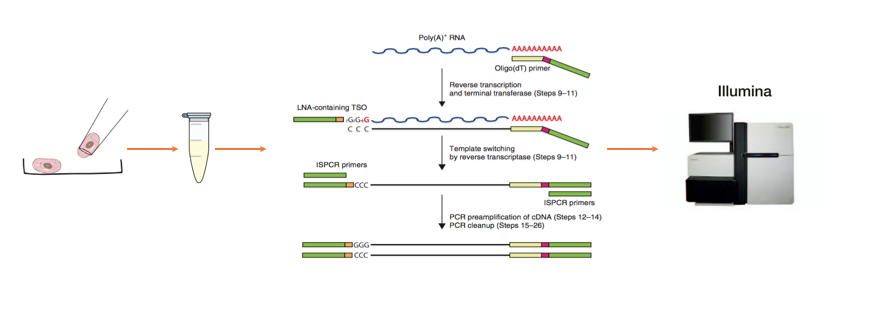
\includegraphics[width=0.8\textwidth]{figs/scseq-smart.png}
  \caption{SMART-seq流程}
  \label{fig:scseq-smart}
\end{figure}

  目前,单细胞RNA测序(scRNA-seq)技术可解决的常见问题\cite{liu2016single,junker2014every}包括:
\begin{itemize}
    \item 探究异质性(Studying heterogeneity)
    \item 谱系路径分析(Lineage tracing study)
    \item 随机基因表达研究(Stochastic gene expression study)
\end{itemize}

\begin{figure}[!htb]
  \centering
  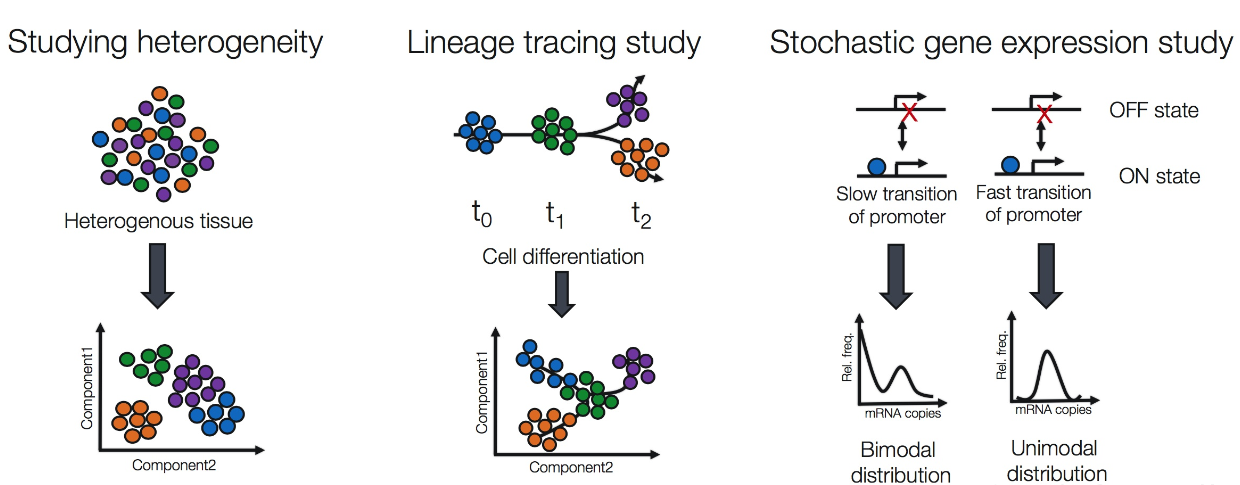
\includegraphics[width=0.8\textwidth]{figs/scseq-purpose.png}
  \caption{单细胞测序可解决的常见问题}
  \label{fig:scseq-purpose}
\end{figure}

\section{垂体在单细胞转录水平的研究}
  以往探究垂体在中枢神经内分泌炎症调节过程中作用的研究\cite{chrousos1995hypothalamic,shanks2000early},表明HPA轴是体内的压力反应中心,垂体积极参与中枢神经内分泌炎症调节过程。但这些研究都没有涉及到单细胞转录层级,没有揭示垂体内部各类细胞在中枢神经内分泌炎症调解过程中的角色以及内在调控因子。近几年,也有一些使用单细胞RNA测序(scRNA-seq)技术研究垂体的工作\cite{chen2020single,cheung2018single,ho2020single,fletcher2019cell},但这些工作主要关注于某个发育过程中的静态分类问题,很少有研究使用单细胞转录组测序来进行动态功能研究。

  这项研究中,我们主要关注不同的垂体细胞如何响应炎症刺激。我们将基于病毒或细菌感染建立炎症小鼠模型,并主要使用单细胞转录组测序以及数据分析和数据挖掘来找出炎症、垂体和激素之间的关系,动态炎症研究将成为我们实验中最重要的部分。

  这项研究可以使我们对人体对病毒或细菌感染的免疫防御具有更清晰的认识。更重要的是,它具有非常重要的临床意义,我们希望获得用于免疫诊断的特定标记。此外,这项研究也可以为我们提供关于单细胞转录组测序技术应用的新思路。

\section{基因调控网络}
  基因调控网络(GRN)定义并维持特定于细胞类型的转录状态,这反过来又是细胞形态和功能的基础。每种细胞类型或稳定状态均由活性转录因子(TF)的特定组合定义,这些转录因子与基因组中的一组顺式调节区域相互作用(与染色质结构相互作用),以产生特定的基因表达谱\cite{fiers2018mapping,arendt2016origin}。活性TF及其靶基因的组合通常表示为GRN。

  揭露GRN是基因组研究领域的主要挑战之一。一旦确定了驱动并维持细胞状态行为的关键调节剂,它们最终就可以用来干扰这些调节程序。实例包括通过Yamanaka等人\cite{takahashi2006induction}提出的TF组合,将成纤维细胞重编程为诱导性多能干细胞(iPS),还有许多其他重编程途径,它们使用TF的特定组合将GRN从一种状态引导到另一种状态\cite{marro2011direct,ieda2010direct},以及最近在癌症治疗中的尝试,其中癌细胞被推入易受特定药物影响的状态\cite{creixell2012navigating,wouters2017decoding}。

  基于大规模转录组和表观基因组数据来计算预测GRNs是一个广泛研究的领域。相关算法包括GENIE3\cite{huynh2010inferring}、GRNBoost2\cite{moerman2019grnboost2}和BEELINE\cite{pratapa2020benchmarking}等。在这项研究中我们主要使用基于GRNBoost2的SCENIC\cite{aibar2017scenic,van2020scalable},进行基因调控网络推断。

\begin{figure}[!htb]
  \centering
  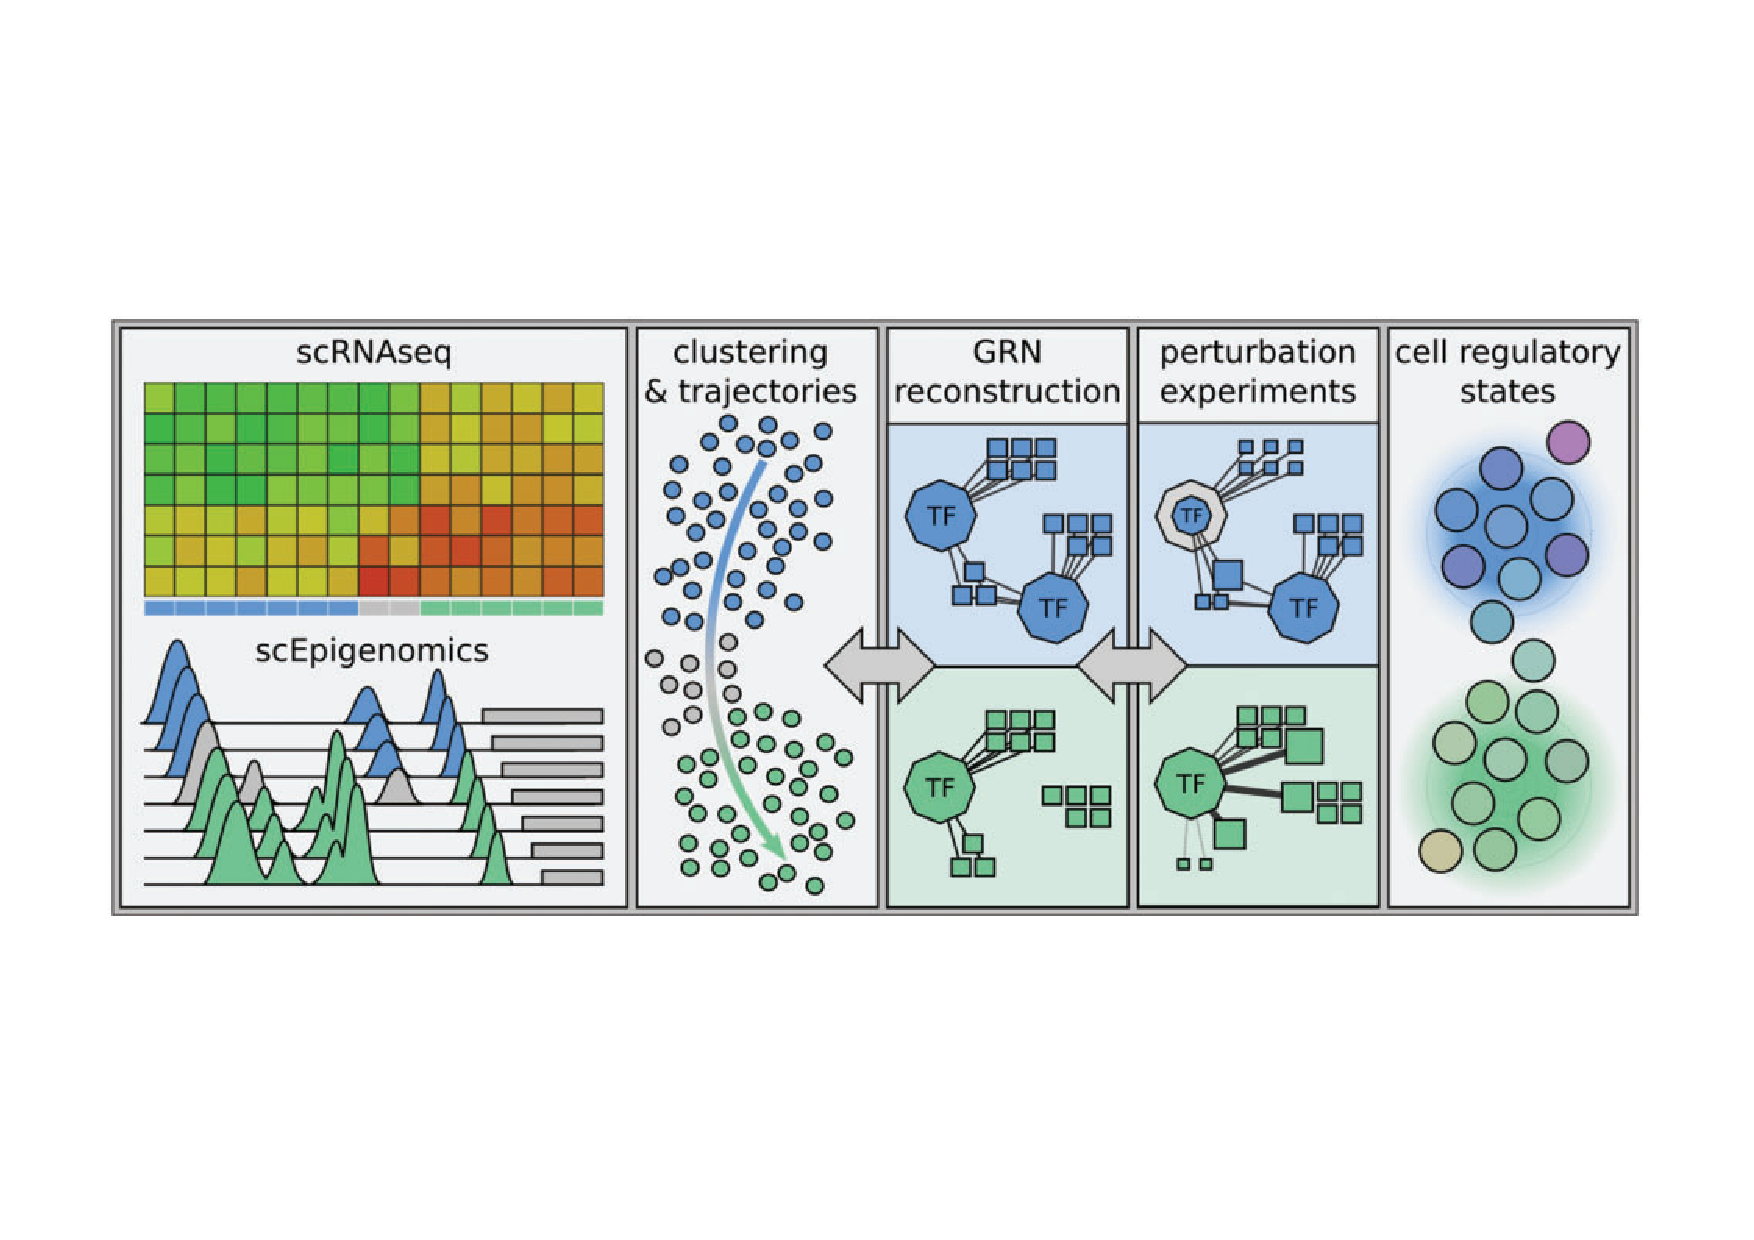
\includegraphics[width=0.9\textwidth]{figs/scgrn-infer.pdf}
  \caption{基因调控网络推断过程}
  \label{fig:scgrn-infer}
\end{figure}

  以往的单细胞RNA测序工作主要使用原始基因表达矩阵进行聚类,进而标记细胞类型以及状态,但结果的真实性经常受到批次效应的挑战。批次效应的产生,是由于涉及单细胞RNA测序的实验往往需要在从多只小鼠上收集数据,而这种操作会引入一些与生物处理无关的噪声(如温度、研磨程度等)。

  相较之下,SCENIC在推导基因调控网络的过程中,能够觉察到一整个基因集合的整体趋势,去除批次效应所带来的影响。此外,SCENIC在推理GRN的时候并不是单纯地依赖GRNBoost2得到的相关性,而是对GRNBoost2推理得到的相关性利用生物学的先验知识进行修剪,只留下具备因果关系的转录因子及其目标基因,能够获得更加生物合理的结果。因而,使用基因调控网络进行聚类,其结果更贴近生物真实状态。

